% -*- mode: latex; mode: flyspell; ispell-local-dictionary: "en_US"; coding: utf-8; fill-column: 80 -*-

\documentclass{article}

\usepackage[utf8]{inputenc}
\usepackage[english]{babel}

\usepackage{amsmath,amsfonts,amssymb}
\usepackage{fullpage}
\usepackage{verbatim}

\usepackage{tikz,pgfplots}

\pgfplotsset{
  width=150mm,height=100mm,
  major grid style={thin,dotted,color=black!50},
  minor grid style={thin,dotted,color=black!50},
  grid,
  every axis/.append style={
    line width=0.5pt,
    tick style={
      line cap=round,
      thin,
      major tick length=4pt,
      minor tick length=2pt,
    },
  },
  legend cell align=left,
  legend pos=north west,
}

%%%%%%%%%%%%%%%%%%%%%%%%%%%%%%%%%%%%%%%%%%%%%%%%%%%%%%%%%%%%%%%%%%%%%%%%%%%%%%%%

\begin{document}

\title{Speicherplatzanalyse Hashmaps}
\author{}
\maketitle


% IMPORT-DATA mphf stats_mphf_size.txt
% IMPORT-DATA hashmap stats_hashmap_size.txt


\begin{center}
	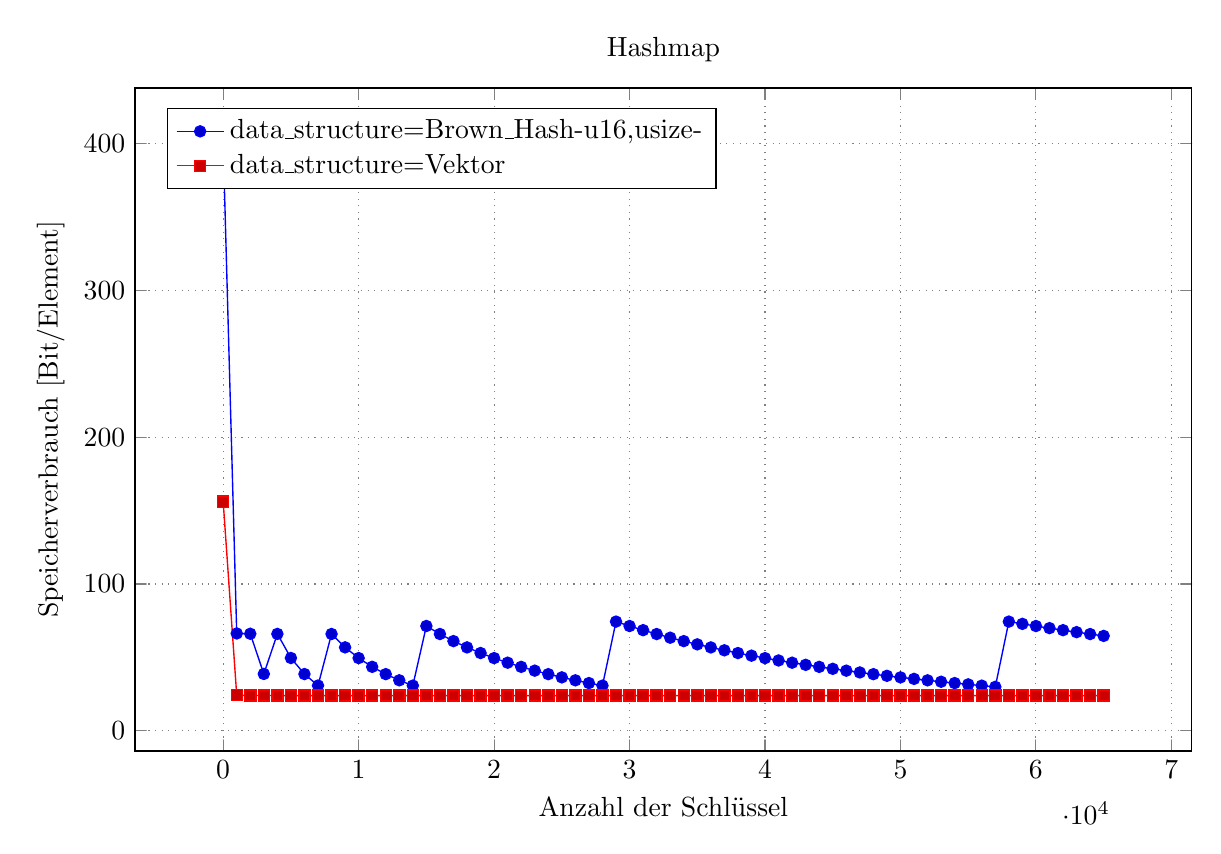
\begin{tikzpicture}
	\begin{axis}[
	title={Hashmap},
	xlabel={Anzahl der Schlüssel},
	ylabel={Speicherverbrauch [Bit/Element]},
	]
	
	%% MULTIPLOT(data_structure) SELECT size AS x, size_bytes AS y, MULTIPLOT
	%% FROM hashmap WHERE x % 1000 == 2  GROUP BY MULTIPLOT,x ORDER BY MULTIPLOT,x
 \addplot coordinates { (2,400.0) (1002,66.3313) (2002,66.1259) (3002,38.7688) (4002,66.023) (5002,49.625) (6002,38.6911) (7002,30.8803) (8002,65.9715) (9002,56.8656) (10002,49.5805) (11002,43.6197) (12002,38.6522) (13002,34.4489) (14002,30.8459) (15002,71.4081) (16002,65.9458) (17002,61.126) (18002,56.8417) (19002,53.0083) (20002,49.5582) (21002,46.4367) (22002,43.5989) (23002,41.0079) (24002,38.6328) (25002,36.4476) (26002,34.4306) (27002,32.5629) (28002,30.8287) (29002,74.4081) (30002,71.3947) (31002,68.5757) (32002,65.9329) (33002,63.4502) (34002,61.1136) (35002,58.9105) (36002,56.8297) (37002,54.8615) (38002,52.9968) (39002,51.2277) (40002,49.5471) (41002,47.9485) (42002,46.426) (43002,44.9743) (44002,43.5886) (45002,42.2644) (46002,40.9979) (47002,39.7852) (48002,38.6231) (49002,37.5083) (50002,36.4382) (51002,35.4101) (52002,34.4214) (53002,33.4701) (54002,32.5541) (55002,31.6713) (56002,30.82) (57002,29.9987) (58002,74.4013) (59002,72.8691) (60002,71.388) (61002,69.9555) (62002,68.5691) (63002,67.2268) (64002,65.9264) (65002,64.6661) };
 \addlegendentry{data\_structure=Brown\_Hash-u16,usize-};
 \addplot coordinates { (2,156.0) (1002,24.2635) (2002,24.1319) (3002,24.0879) (4002,24.066) (5002,24.0528) (6002,24.044) (7002,24.0377) (8002,24.033) (9002,24.0293) (10002,24.0264) (11002,24.024) (12002,24.022) (13002,24.0203) (14002,24.0189) (15002,24.0176) (16002,24.0165) (17002,24.0155) (18002,24.0147) (19002,24.0139) (20002,24.0132) (21002,24.0126) (22002,24.012) (23002,24.0115) (24002,24.011) (25002,24.0106) (26002,24.0102) (27002,24.0098) (28002,24.0094) (29002,24.0091) (30002,24.0088) (31002,24.0085) (32002,24.0082) (33002,24.008) (34002,24.0078) (35002,24.0075) (36002,24.0073) (37002,24.0071) (38002,24.0069) (39002,24.0068) (40002,24.0066) (41002,24.0064) (42002,24.0063) (43002,24.0061) (44002,24.006) (45002,24.0059) (46002,24.0057) (47002,24.0056) (48002,24.0055) (49002,24.0054) (50002,24.0053) (51002,24.0052) (52002,24.0051) (53002,24.005) (54002,24.0049) (55002,24.0048) (56002,24.0047) (57002,24.0046) (58002,24.0046) (59002,24.0045) (60002,24.0044) (61002,24.0043) (62002,24.0043) (63002,24.0042) (64002,24.0041) (65002,24.0041) };
 \addlegendentry{data\_structure=Vektor};
 

	
	
	\end{axis}
	\end{tikzpicture}
\end{center}


\begin{center}
	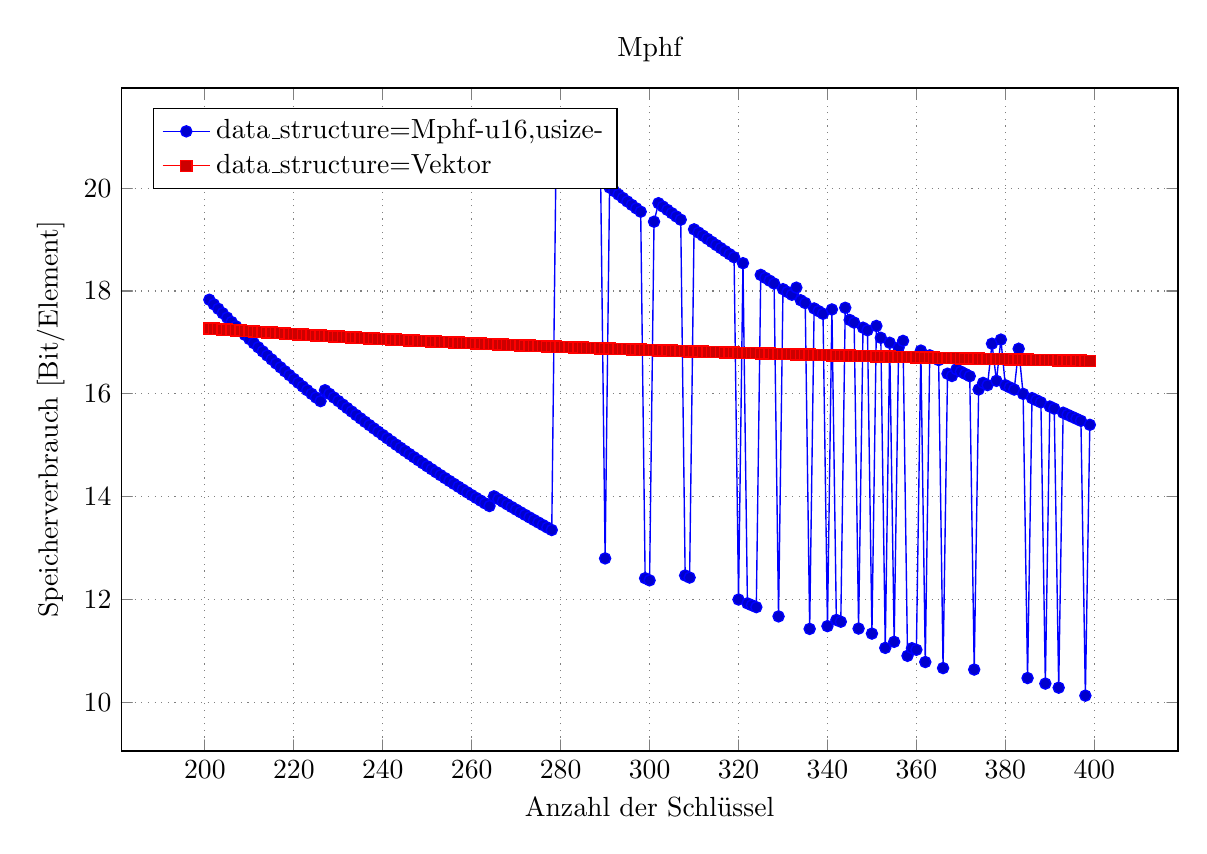
\begin{tikzpicture}
	\begin{axis}[
	title={Mphf},
	xlabel={Anzahl der Schlüssel},
	ylabel={Speicherverbrauch [Bit/Element]},
	]
	
	%% MULTIPLOT(data_structure) SELECT size AS x, size_bytes AS y, MULTIPLOT
	%% FROM mphf WHERE  x > 200 AND x < 400 GROUP BY MULTIPLOT,x ORDER BY MULTIPLOT,x
 \addplot coordinates { (201,17.8308) (202,17.7426) (203,17.6552) (204,17.5686) (205,17.4829) (206,17.3981) (207,17.314) (208,17.2308) (209,17.1483) (210,17.0667) (211,16.9858) (212,16.9057) (213,16.8263) (214,16.7477) (215,16.6698) (216,16.5926) (217,16.5161) (218,16.4404) (219,16.3653) (220,16.2909) (221,16.2172) (222,16.1441) (223,16.0717) (224,16.0) (225,15.9289) (226,15.8584) (227,16.0705) (228,16.0) (229,15.9301) (230,15.8609) (231,15.7922) (232,15.7241) (233,15.6567) (234,15.5897) (235,15.5234) (236,15.4576) (237,15.3924) (238,15.3277) (239,15.2636) (240,15.2) (241,15.1369) (242,15.0744) (243,15.0123) (244,14.9508) (245,14.8898) (246,14.8293) (247,14.7692) (248,14.7097) (249,14.6506) (250,14.592) (251,14.5339) (252,14.4762) (253,14.419) (254,14.3622) (255,14.3059) (256,14.25) (257,14.1946) (258,14.1395) (259,14.0849) (260,14.0308) (261,13.977) (262,13.9237) (263,13.8707) (264,13.8182) (265,14.0075) (266,13.9549) (267,13.9026) (268,13.8507) (269,13.7993) (270,13.7481) (271,13.6974) (272,13.6471) (273,13.5971) (274,13.5474) (275,13.4982) (276,13.4493) (277,13.4007) (278,13.3525) (279,20.8746) (280,20.8) (281,20.726) (282,20.6525) (283,20.5795) (284,20.507) (285,20.4351) (286,20.3636) (287,20.2927) (288,20.2222) (289,20.1522) (290,12.8) (291,20.0137) (292,19.9452) (293,19.8771) (294,19.8095) (295,19.7424) (296,19.6757) (297,19.6094) (298,19.5436) (299,12.4147) (300,12.3733) (301,19.3488) (302,19.7086) (303,19.6436) (304,19.5789) (305,19.5148) (306,19.451) (307,19.3876) (308,12.4675) (309,12.4272) (310,19.2) (311,19.1383) (312,19.0769) (313,19.016) (314,18.9554) (315,18.8952) (316,18.8354) (317,18.776) (318,18.717) (319,18.6583) (320,12.0) (321,18.5421) (322,11.9255) (323,11.8885) (324,11.8519) (325,18.3138) (326,18.2577) (327,18.2018) (328,18.1463) (329,11.6717) (330,18.0364) (331,17.9819) (332,17.9277) (333,18.0661) (334,17.8204) (335,17.7672) (336,11.4286) (337,17.6617) (338,17.6095) (339,17.5575) (340,11.4824) (341,17.6422) (342,11.6023) (343,11.5685) (344,17.6744) (345,17.4377) (346,17.3873) (347,11.4352) (348,17.2874) (349,17.2378) (350,11.3371) (351,17.3219) (352,17.0909) (353,11.0595) (354,16.9944) (355,11.1775) (356,16.8989) (357,17.0308) (358,10.905) (359,11.0529) (360,11.0222) (361,16.8421) (362,10.7845) (363,16.7493) (364,16.7033) (365,16.6575) (366,10.6667) (367,16.3924) (368,16.3478) (369,16.477) (370,16.4324) (371,16.3881) (372,16.3441) (373,10.6381) (374,16.0856) (375,16.2133) (376,16.1702) (377,16.9761) (378,16.254) (379,17.0554) (380,16.1684) (381,16.126) (382,16.0838) (383,16.8773) (384,16.0) (385,10.4727) (386,15.9171) (387,15.876) (388,15.8351) (389,10.365) (390,15.7538) (391,15.7136) (392,10.2857) (393,15.6336) (394,15.5939) (395,15.5544) (396,15.5152) (397,15.4761) (398,10.1307) (399,15.3985) };
 \addlegendentry{data\_structure=Mphf-u16,usize-};
 \addplot coordinates { (201,17.2736) (202,17.2673) (203,17.2611) (204,17.2549) (205,17.2488) (206,17.2427) (207,17.2367) (208,17.2308) (209,17.2249) (210,17.219) (211,17.2133) (212,17.2075) (213,17.2019) (214,17.1963) (215,17.1907) (216,17.1852) (217,17.1797) (218,17.1743) (219,17.1689) (220,17.1636) (221,17.1584) (222,17.1532) (223,17.148) (224,17.1429) (225,17.1378) (226,17.1327) (227,17.1278) (228,17.1228) (229,17.1179) (230,17.113) (231,17.1082) (232,17.1034) (233,17.0987) (234,17.094) (235,17.0894) (236,17.0847) (237,17.0802) (238,17.0756) (239,17.0711) (240,17.0667) (241,17.0622) (242,17.0579) (243,17.0535) (244,17.0492) (245,17.0449) (246,17.0407) (247,17.0364) (248,17.0323) (249,17.0281) (250,17.024) (251,17.0199) (252,17.0159) (253,17.0119) (254,17.0079) (255,17.0039) (256,17.0) (257,16.9961) (258,16.9922) (259,16.9884) (260,16.9846) (261,16.9808) (262,16.9771) (263,16.9734) (264,16.9697) (265,16.966) (266,16.9624) (267,16.9588) (268,16.9552) (269,16.9517) (270,16.9481) (271,16.9446) (272,16.9412) (273,16.9377) (274,16.9343) (275,16.9309) (276,16.9275) (277,16.9242) (278,16.9209) (279,16.9176) (280,16.9143) (281,16.911) (282,16.9078) (283,16.9046) (284,16.9014) (285,16.8982) (286,16.8951) (287,16.892) (288,16.8889) (289,16.8858) (290,16.8828) (291,16.8797) (292,16.8767) (293,16.8737) (294,16.8707) (295,16.8678) (296,16.8649) (297,16.862) (298,16.8591) (299,16.8562) (300,16.8533) (301,16.8505) (302,16.8477) (303,16.8449) (304,16.8421) (305,16.8393) (306,16.8366) (307,16.8339) (308,16.8312) (309,16.8285) (310,16.8258) (311,16.8232) (312,16.8205) (313,16.8179) (314,16.8153) (315,16.8127) (316,16.8101) (317,16.8076) (318,16.805) (319,16.8025) (320,16.8) (321,16.7975) (322,16.795) (323,16.7926) (324,16.7901) (325,16.7877) (326,16.7853) (327,16.7829) (328,16.7805) (329,16.7781) (330,16.7758) (331,16.7734) (332,16.7711) (333,16.7688) (334,16.7665) (335,16.7642) (336,16.7619) (337,16.7596) (338,16.7574) (339,16.7552) (340,16.7529) (341,16.7507) (342,16.7485) (343,16.7464) (344,16.7442) (345,16.742) (346,16.7399) (347,16.7378) (348,16.7356) (349,16.7335) (350,16.7314) (351,16.7293) (352,16.7273) (353,16.7252) (354,16.7232) (355,16.7211) (356,16.7191) (357,16.7171) (358,16.7151) (359,16.7131) (360,16.7111) (361,16.7091) (362,16.7072) (363,16.7052) (364,16.7033) (365,16.7014) (366,16.6995) (367,16.6975) (368,16.6957) (369,16.6938) (370,16.6919) (371,16.69) (372,16.6882) (373,16.6863) (374,16.6845) (375,16.6827) (376,16.6809) (377,16.679) (378,16.6772) (379,16.6755) (380,16.6737) (381,16.6719) (382,16.6702) (383,16.6684) (384,16.6667) (385,16.6649) (386,16.6632) (387,16.6615) (388,16.6598) (389,16.6581) (390,16.6564) (391,16.6547) (392,16.6531) (393,16.6514) (394,16.6497) (395,16.6481) (396,16.6465) (397,16.6448) (398,16.6432) (399,16.6416) };
 \addlegendentry{data\_structure=Vektor};

 
	
	\end{axis}
	\end{tikzpicture}
\end{center}


\end{document}

%%%%%%%%%%%%%%%%%%%%%%%%%%%%%%%%%%%%%%%%%%%%%%%%%%%%%%%%%%%%%%%%%%%%%%%%%%%%%%%%
